\documentclass{tp}
\titre{TP17 : Le goniomètre}
\begin{document}
%\small

\section{Objectif du TP}
Le but de ce TP est d'apprendre à utiliser un goniomètre. C'est un instrument qui permet de faire des mesures d'angles précises. On l'utilisera avec un réseau pour mesurer les longueurs d'onde d'une lampe spectrale.

\section{La lampe spectrale}%
\label{sec:la_lampe_spectrale}
Une lampe spectrale est une ampoule contenant un gaz dans lequel on fait passer un courant électrique. Cela a pour effet d'exciter les atomes du gaz qui émettent de la lumière lorsqu'ils se désexcitent. Vous disposez d'une lampe au mercure et d'une lampe au sodium. Quelques précautions sont à prendre avec la lampe au mercure :

\begin{itemize}
  \item La lampe spectrale au mercure émet de la lumière ultraviolette. Il ne faut pas la regarder directement. Lorsqu'elle est allumée il faut autant que possible cacher la lumière qui ne passe pas dans le système optique. Par contre il n'y a pas de risque à la regarder à travers un système optique constitué de plusieurs lentilles car le verre absorbe les UV.

  \item Les cycles allumage/extinction ne sont pas très bons pour la lampe, on veillera donc à éviter de l'éteindre une fois qu'elle est allumée.

  \item Si la lampe s'éteint, on attendra 5 minutes avant de la rallumer.
\end{itemize}

\section{Le goniomètre}

\noindent Les mesures d'angles sont réalisées à l'aide d'un \textbf{goniomètre} (Du grec << gonio >>, $\equiv$ << angle >>). Celui-ci est composé de trois parties :
\vspace{0.1cm}

\begin{itemize}
	\item[$\bullet$] une \textbf{plate-forme} sur laquelle on place le réseau utilisé ;
	\item[$\bullet$] un \textbf{collimateur à fente}, qui permet de réaliser un faisceau de lumière parallèle en plaçant une fente dans le plan focal objet d'une lentille convergente ;
	\item[$\bullet$] une \textbf{lunette d'observation}, mobile par rapport à la plate-forme, permet de mesurer les directions des faisceaux parallèles incidents en observant des objets situés à l'infini.
\end{itemize}

\subsection{La lunette d'observation}
La lunette d'observation comporte un objectif (lentille convergente), un réticule (un objet en forme de croix) et un oculaire (doublet de lentilles).

Le réticule est fixé sur la monture de la lunette, on peut régler son orientation et on peut ajuster les positions de l'objectif et de l'oculaire.

La lunette possède aussi un éclairage latéral qui permet d'éclairer le réticule. Ainsi qu'une lame semi-réfléchissante que l'on peut positionner soit pour éclairer uniquement le réticule, soit pour envoyer la lumière à travers le réticule et le reste de la lunette.

\begin{center}
  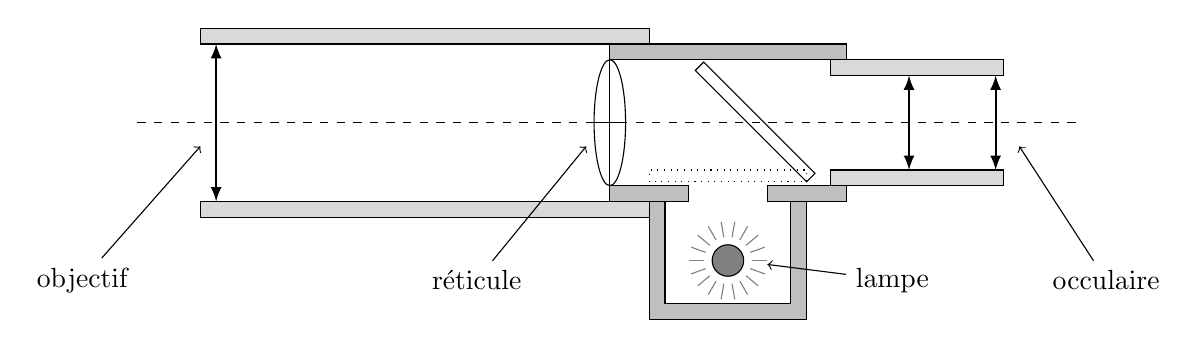
\begin{tikzpicture}
    \draw[dashed] (0,0)  -- (12,0);
    \draw[latex-latex, thick] (1,-1) -- (1, 1); %Objectif
    \draw[fill=gray!30] (0.8,1) rectangle (6.5, 1.2);
    \draw[fill=gray!30] (0.8,-1) rectangle (6.5, -1.2);

    %réticule
    \draw (6,0) circle[x radius=2mm, y radius=0.8cm];
    \draw (5.8, 0) -- (6.2,0);
    \draw (6,-0.8) -- (6, 0.8);

    \draw[fill=gray!50] (6,0.8) rectangle (9, 1);
    \draw[fill=gray!50] (6,-0.8) rectangle (7, -1);
    \draw[fill=gray!50] (8,-0.8) rectangle (9, -1);

    \draw[fill=gray!50] (6.5,-1) -- ++(0, -1.5) -- ++(2, 0) -- ++(0, 1.5) -- ++ (-0.2, 0) -- ++ (0, -1.3) -- ++(-1.6, 0) -- ++(0, 1.3) -- cycle;

    \draw[fill=gray] (7.5, -1.75) circle (0.2);
    \foreach \angle in {0,20,...,340}{
      \draw[gray] (7.5, -1.75) ++ (\angle:0.3) -- ++(\angle:0.2);
    }

    \draw[dotted] (6.5, -0.75) rectangle (8.5, -0.6);
    \begin{scope}[rotate around={-45:(8.5, -0.75)}]
      \draw[] (6.5, -0.75) rectangle (8.5, -0.6);
    \end{scope}

    \draw[fill=gray!30] (8.8, -0.8) rectangle (11, -0.6);
    \draw[fill=gray!30] (8.8, 0.8) rectangle (11, 0.6);

    \draw[latex-latex, thick] (9.8,-0.6) -- (9.8, 0.6); %Objectif
    \draw[latex-latex, thick] (10.9,-0.6) -- (10.9, 0.6); %Objectif

    \draw (5, -2) node[left] (reticule) {réticule};
    \draw[->] (reticule) -- (5.7, -0.3);

    \draw (0, -2) node[left] (objectif) {objectif};
    \draw[->] (objectif) -- (0.8, -0.3);

    \draw (11.5, -2) node[right] (occulaire) {occulaire};
    \draw[->] (occulaire) -- (11.2, -0.3);

    \draw (9, -2) node[right] (lampe) {lampe};
    \draw[->] (lampe) -- (8, -1.8);
  \end{tikzpicture}
\end{center}

Pour régler correctement la lunette on procédera aux étapes suivantes :
\begin{itemize}
  \item \textbf{Réglage de l’oculaire : } Il s’agit de régler la distance oculaire-réticule pour voir le réticule net sans accommodation : si l’on regarde d’abord (à l’\oe{}il nu) un objet lointain, l’\oe{}il doit ensuite voir directement net le réticule (sans temps d’accommodation). Pour l’\oe{}il emmétrope ou bien corrigé, le réticule est alors dans le plan focal objet de l’oculaire.

Ce réglage est \emph{subjectif}, il doit être modifié à chaque changement d’observateur.

\item \textbf{Réglage de l’objectif : } Il consiste à faire coïncider le plan focal image de l'objectif et le plan du réticule. On procède par autocollimation, grâce au dispositif d’éclairage du réticule, et à un miroir plan que l’on placera devant la lunette. En observant dans l’oculaire, régler l’objectif de sorte que le réticule et son image soient dans le même plan : ils sont alors nets simultanément, et ne bougent pas l’un par rapport à l’autre si l’on déplace latéralement l’\oe{}il devant
l’oculaire.

Ce réglage est \emph{objectif}, il sera donc fait une fois pour toutes et pourra être contrôlé par n’importe quel observateur ayant préalablement réglé l’oculaire à sa vue.
\end{itemize}

Le réglage de la lunette doit être effectué au moins une fois par chaque membre du groupe et vérifié par le(s) autre(s) membre(s).

\subsection{Le collimateur}

Le collimateur permet de créer un faisceau de rayons parallèles à partir d'une source lumineuse, il est composé d'une fente de largeur réglable devant laquelle on place la source lumineuse et d'un objectif dont on peut ajuster la distance à la fente.

Pour régler le collimateur, on utilise le fait que la lunette est déjà réglée pour former dans le plan du réticule l'image d'objets se situant à l'infini. On place donc une lumière blanche devant la fente et on diminue autant que possible la largeur de la fente. On règle ensuite la distance fente-objectif pour observer une image nette de la fente à travers la lunette.

Encore une fois, chaque membre du groupe de TP doit effectuer ce réglage au moins une fois.

\subsection{Utilisation du goniomètre}
Dans le goniomètre, le collimateur est fixe et la lunette d'observation est mobile, on peut faire varier l'angle entre sa direction d'observation et la direction des rayons émis par le collimateur.

\textbf{Attention : Le goniomètre ne permet pas de mesurer des angles absolus mais seulement des différences d'angles. Il faut définir une direction de référence.}

On peut également faire tourner la plate-forme mobile pour modifier l'angle d'incidence des rayons sur l'objet étudié.

\section{Mesures de longueurs d'onde}
Vous disposez d'une lampe spectrale au mercure. C'est une lampe qui utilise les transitions entre différents niveaux atomiques pour émettre de la lumière. Le spectre émis est un spectre de raies. 

Nous allons commencer par mesurer les longueurs d'onde des différentes raies émises par la lampe.

\subsection{Le réseau}
\begin{minipage}{0.4\linewidth}
%\includegraphics[width=0.9\linewidth]{TP7_reseau.pdf}
\begin{tikzpicture}[rayon/.style = {postaction={decorate},decoration = {markings, mark = at position 0.5 with {\arrow{latex}}}}
]
\draw[-Latex] (0,0) -- (6,0);
\draw[dotted,|-|] (3,-1) -- (3,1) node[above,align=center]{Réseau};
\foreach \h in {-0.7,-0.2,0.2,0.7}{
  \draw[rayon] (0,\h) -- (3,\h) ;
  \draw[rayon] (3,\h) -- ++(20:3);
}
\draw (4.5,0) arc (0:20:0.9) node[midway, right] {$\theta$};
\draw (1.5,-0.7) node[below,align=center] {\small Faisceau incident\\parallèle};
\end{tikzpicture}

\end{minipage}
\begin{minipage}{0.6\linewidth}
Pour mesurer les longueurs d'onde émises par la lampe spectrale, on utilise un réseau de diffraction. C'est un objet transparent sur lequel on a ajouté un grand nombre de \textit{traits} opaques. Le réseau est caractérisé par son nombre de traits par millimètre $n$.
\end{minipage}
Un réseau a la propriété de disperser la lumière incidente, c'est à dire qu'un rayon lumineux sera dévié d'un angle $\theta$ qui dépend de sa longueur d'onde $\lambda$. L'angle $\theta$ est donné par la formule :
\begin{equation*}
	\sin(\theta) = p\dfrac{\lambda}{a}
\end{equation*}
où $a$ est le \textit{pas} du réseau, c'est à dire la distance qui sépare deux traits opaques, et $p$ est un nombre entier relatif appelé \emph{ordre d'interférence}. 

Comme il y a plusieurs valeurs de $p$ possible, un faisceau incident sera dévié dans plusieurs directions différentes. En pratique on pourra observer les ordres $p=-2, -1, 0, 1, 2$.

Ainsi en mesurant la déviation $\theta$ pour un ordre de diffraction $p$ de la lumière, on peut en déterminer sa longueur d'onde $\lambda$.  

Pour toutes les mesures, on veillera à ce que le réseau soit parfaitement perpendiculaire au faisceau incident. Pour cela on pourra procéder de la manière suivante :
\begin{itemize}
  \item Régler l'orientation de la lunette pour que l'image de la fente du collimateur soit parfaitement centrée sur le réticule. Bloquer alors l'orientation de la lunette
  \item Insérer le réseau sur la platine et le positionner perpendiculairement à l'axe collimateur-lunette. Bloquer la rotation de la platine.
  \item Éclairer le réseau avec la lampe de la lunette, une partie de la lumière se réfléchie vers la lunette. Tourner la vis de réglage fin de la rotation de la platine pour superposer le réticule à son image. Le réseau est alors parfaitement perpendiculaire au collimateur.
  \item Débloquer la rotation de la lunette.
\end{itemize}

\subsection{Mesures}
\begin{itemize}[resume=TP]
\item Utiliser un réseau de diffraction pour déterminer aussi précisément que possible les longueurs d'onde émises par la lampe spectrale au mercure

\item Comparer les valeurs obtenues avec celles qui se trouvent dans l'annexe ci-dessous.

\item Si le temps le permet, utiliser le montage pour observer le doublet jaune du sodium (deux raies très proches l'une de l'autre).
\end{itemize}

 %\pagebreak
 \section{Annexe}%
 \label{sec:annexe}

 On donne dans les tableaux ci-dessous les valeurs de quelques raies des lampes spectrales utilisées. 

\vspace{1em}

 \noindent \begin{minipage}{0.5\linewidth}
  \begin{center}
   \begin{tabular}{@{}ll@{}}
     \toprule
     Longueur d'onde (nm) & couleur \\
     \midrule
     404.657 & \definecolor{violet}{HTML}{8200C4} \tikz[baseline=1pt] \fill[violet] (0,0) rectangle (1em,1em); violet \\
     407.784 & \definecolor{violet}{HTML}{8200C4} \tikz[baseline=1pt] \fill[violet] (0,0) rectangle (1em,1em); violet \\
     435.834 & \definecolor{bleu}{HTML}{2300FF} \tikz[baseline=1pt] \fill[bleu] (0,0) rectangle (1em,1em); bleu \\
     491.607 & \definecolor{vertclair}{HTML}{00FFCB} \tikz[baseline=1pt] \fill[vertclair] (0,0) rectangle (1em,1em); vert clair \\
     546.075 & \definecolor{vertjaune}{HTML}{96FF00} \tikz[baseline=1pt] \fill[vertjaune] (0,0) rectangle (1em,1em); vert/jaune \\
     576.961 et 579.067 & \definecolor{jaune}{HTML}{F6FF00} \tikz[baseline=1pt] \fill[jaune] (0,0) rectangle (1em,1em); jaune (doublet) \\
     \bottomrule
   \end{tabular}
   \captionof{table}{Quelques raies d'une lampe au mercure. Source : \url{https://physics.nist.gov/PhysRefData/Handbook/Tables/mercurytable2.htm}}
   \end{center}
   \end{minipage}%
   \begin{minipage}{0.5\linewidth}
   \begin{center}
   \begin{tabular}{@{}ll@{}}
     \toprule
     Longueur d'onde (nm) & couleur \\
     \midrule
     449.1 & \definecolor{bleu}{HTML}{2300FF} \tikz[baseline=1pt] \fill[bleu] (0,0) rectangle (1em,1em); bleu \\
     588.995 & \definecolor{orange}{HTML}{FFE200} \tikz[baseline=1pt] \fill[orange] (0,0) rectangle (1em,1em); orange \\
     589.592 & \definecolor{orange}{HTML}{FFE200} \tikz[baseline=1pt] \fill[orange] (0,0) rectangle (1em,1em); orange \\
     653.1 & \definecolor{rouge}{HTML}{FF0000} \tikz[baseline=1pt] \fill[rouge] (0,0) rectangle (1em,1em); rouge \\
     \bottomrule
   \end{tabular}
   \captionof{table}{Quelques raies d'une lampe au sodium. Source : \url{https://physics.nist.gov/PhysRefData/Handbook/Tables/sodiumtable2.htm}}
 \end{center}
 \end{minipage}

\vspace{2em}

\vspace{1cm}
On montre également ci-dessous comment lire les graduations du \textit{vernier} du goniomètre.
\begin{center}
  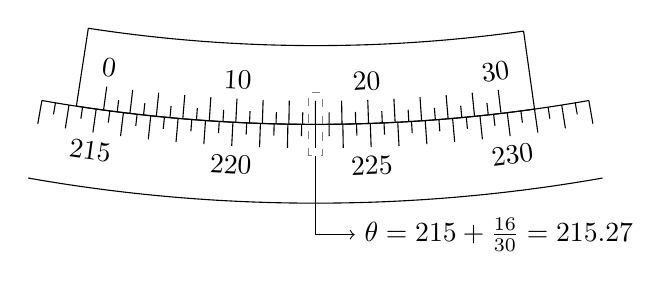
\begin{tikzpicture}
    \draw (-100:20) arc (-100:-80:20);
    \draw (-100:21) arc (-100:-80:21);
    \foreach \a in {-100, -99,..., -80}{
      \draw (\a:20) -- (\a: 20.3);
    }
    \foreach \a in {-100, -99,..., -81}{
      \draw (\a+0.5:20) -- (\a+0.5: 20.15);
    }
    \draw (-98:20.3) node[below, rotate=-8]{215};
    \draw (-93:20.3) node[below, rotate=-3]{220};
    \draw (-88:20.3) node[below, rotate=2]{225};
    \draw (-83:20.3) node[below, rotate=7]{230};

    \draw (-98.73:20) arc (-98.73:-82:20);
    \draw (-98.73:19) arc (-98.73:-82:19);
    \draw (-98.73:20) -- (-98.73:19);
    \draw (-82:20) -- (-82:19);
    \foreach \i in{0, 1,...,15}{
      \draw (-97.73+\i*29/30:20) -- (-97.73+\i*29/30:19.7);
    }
    \foreach \i in{0, 1,...,14}{
      \draw (-97.73+\i*29/30+0.5:20) -- (-97.73+\i*29/30+0.5:19.85);
    }
    \draw (-97.73:19.7) node[above, rotate=-7.73] {$0$}; 
    \draw (-97.73+5*29/30:19.7) node[above, rotate=-2.73+1/6] {$10$}; 
    \draw (-97.73+10*29/30:19.7) node[above, rotate=3.27+2/6] {$20$}; 
    \draw (-97.73+15*29/30:19.7) node[above, rotate=8.27+3/6] {$30$}; 
   
    \draw[dashed, gray](-90.25:20.4) rectangle (-89.75:19.6);
    \draw[->] (-90:20.4) -- ++(0, -1) -- ++(0.5, 0) node[right] {$\theta = 215 + \frac{16}{30} = \SI{215.27}{\degree}$ };
  \end{tikzpicture}
\end{center}

\begin{center}
  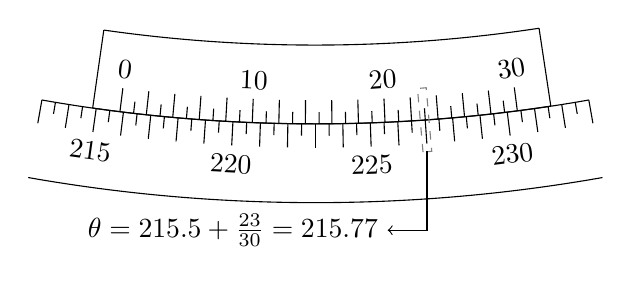
\begin{tikzpicture}
    \draw (-100:20) arc (-100:-80:20);
    \draw (-100:21) arc (-100:-80:21);
    \foreach \a in {-100, -99,..., -80}{
      \draw (\a:20) -- (\a: 20.3);
    }
    \foreach \a in {-100, -99,..., -81}{
      \draw (\a+0.5:20) -- (\a+0.5: 20.15);
    }
    \draw (-98:20.3) node[below, rotate=-8]{215};
    \draw (-93:20.3) node[below, rotate=-3]{220};
    \draw (-88:20.3) node[below, rotate=2]{225};
    \draw (-83:20.3) node[below, rotate=7]{230};

    \draw (-98.13:20) arc (-98.13:-81.4:20);
    \draw (-98.13:19) arc (-98.13:-81.4:19);
    \draw (-98.13:20) -- (-98.13:19);
    \draw (-81.4:20) -- (-81.4:19);
    \foreach \i in{0, 1,...,15}{
      \draw (-97.13+\i*29/30:20) -- (-97.13+\i*29/30:19.7);
    }
    \foreach \i in{0, 1,...,14}{
      \draw (-97.13+\i*29/30+0.5:20) -- (-97.13+\i*29/30+0.5:19.85);
    }
    \draw (-97.13:19.7) node[above, rotate=-7.13] {$0$}; 
    \draw (-97.13+5*29/30:19.7) node[above, rotate=-2.13+1/6] {$10$}; 
    \draw (-97.13+10*29/30:19.7) node[above, rotate=3.87+2/6] {$20$}; 
    \draw (-97.13+15*29/30:19.7) node[above, rotate=8.87+3/6] {$30$}; 
   
    \draw[dashed, gray, rotate around={5:(-97.13+11.5*29/30:20.4)}](-97.13+11.35*29/30:20.4) rectangle (-97.13+11.85*29/30:19.6);
    \draw[->] (-97.13+11.5*29/30:20.4) -- ++(0, -1) -- ++(-0.5, 0) node[left] {$\theta = \num{215.5} + \frac{23}{30} = \SI{215.77}{\degree}$ };
  \end{tikzpicture}
\end{center}
 %\section{\'Etude du prisme}
%On se propose d'utiliser le goniomètre pour étudier la déviation de la lumière par un prisme. On place un prisme d'angle au sommet $A$ sur la plate-forme du goniomètre.

%\subsection{Mesure de l'angle au sommet du prisme}
%\begin{minipage}{0.4\linewidth}
%\includegraphics[width=\linewidth]{TP7_angle_prisme.pdf}
%\end{minipage}
%\begin{minipage}{0.57\linewidth}
%\begin{enumerate}[resume=TP]
	%\item Faire arriver un faisceau de rayons parallèles sur l'angle du prisme et mesurer l'angle $A'$ entre les deux faisceaux réfléchis. 

	%\item On peut montrer que $A'=2A$. En déduire l'angle au somment du prisme.
%\end{enumerate}
%\end{minipage}

%\subsection{Mesure de l'indice du prisme pour différentes longueurs d'onde}
%On peut montrer que la déviation $D$ subie par un faisceau lumineux incident sur le prisme varie en fonction de l'angle d'incidence en passant par une valeur minimale $D_m$. De la mesure de l'angle de déviation minimale $D_m$ on peut déduire l'indice optique du prisme par la formule 
%\begin{equation}
	%n\sin\left(\frac{A}{2}\right) = \sin\left(\frac{D_m+A}{2}\right)
%\end{equation}
%\begin{enumerate}[resume=TP]
	%\item Mesurer pour différentes longueurs d'onde l'angle de déviation minimale $D_m$ et en déduire l'indice optique du prisme à la longueur d'onde en question.

	%\item Tracer l'évolution de l'indice optique du prisme en fonction de $\lambda$ puis en fonction de $A/\lambda^2$. Commenter.
%\end{enumerate}
\end{document}
